
%% bare_jrnl_compsoc.tex
%% V1.4
%% 2012/12/27
%% by Michael Shell
%% See:
%% http://www.michaelshell.org/
%% for current contact information.
%%
%% This is a skeleton file demonstrating the use of IEEEtran.cls
%% (requires IEEEtran.cls version 1.8 or later) with an IEEE Computer
%% Society journal paper.
%%
%% Support sites:
%% http://www.michaelshell.org/tex/ieeetran/
%% http://www.ctan.org/tex-archive/macros/latex/contrib/IEEEtran/
%% and
%% http://www.ieee.org/

%%*************************************************************************
%% Legal Notice:
%% This code is offered as-is without any warranty either expressed or
%% implied; without even the implied warranty of MERCHANTABILITY or
%% FITNESS FOR A PARTICULAR PURPOSE! 
%% User assumes all risk.
%% In no event shall IEEE or any contributor to this code be liable for
%% any damages or losses, including, but not limited to, incidental,
%% consequential, or any other damages, resulting from the use or misuse
%% of any information contained here.
%%
%% All comments are the opinions of their respective authors and are not
%% necessarily endorsed by the IEEE.
%%
%% This work is distributed under the LaTeX Project Public License (LPPL)
%% ( http://www.latex-project.org/ ) version 1.3, and may be freely used,
%% distributed and modified. A copy of the LPPL, version 1.3, is included
%% in the base LaTeX documentation of all distributions of LaTeX released
%% 2003/12/01 or later.
%% Retain all contribution notices and credits.
%% ** Modified files should be clearly indicated as such, including  **
%% ** renaming them and changing author support contact information. **
%%
%% File list of work: IEEEtran.cls, IEEEtran_HOWTO.pdf, bare_adv.tex,
%%                    bare_conf.tex, bare_jrnl.tex, bare_jrnl_compsoc.tex,
%%                    bare_jrnl_transmag.tex
%%*************************************************************************

% *** Authors should verify (and, if needed, correct) their LaTeX system  ***
% *** with the testflow diagnostic prior to trusting their LaTeX platform ***
% *** with production work. IEEE's font choices can trigger bugs that do  ***
% *** not appear when using other class files.                            ***
% The testflow support page is at:
% http://www.michaelshell.org/tex/testflow/




% Note that the a4paper option is mainly intended so that authors in
% countries using A4 can easily print to A4 and see how their papers will
% look in print - the typesetting of the document will not typically be
% affected with changes in paper size (but the bottom and side margins will).
% Use the testflow package mentioned above to verify correct handling of
% both paper sizes by the user's LaTeX system.
%
% Also note that the "draftcls" or "draftclsnofoot", not "draft", option
% should be used if it is desired that the figures are to be displayed in
% draft mode.
%
% The Computer Society usually requires 12pt for submissions.
%
\documentclass[12pt,journal,compsoc]{IEEEtran}
%
% If IEEEtran.cls has not been installed into the LaTeX system files,
% manually specify the path to it like:
% \documentclass[12pt,journal,compsoc]{../sty/IEEEtran}





% Some very useful LaTeX packages include:
% (uncomment the ones you want to load)


% *** MISC UTILITY PACKAGES ***
%
%\usepackage{ifpdf}
% Heiko Oberdiek's ifpdf.sty is very useful if you need conditional
% compilation based on whether the output is pdf or dvi.
% usage:
% \ifpdf
%   % pdf code
% \else
%   % dvi code
% \fi
% The latest version of ifpdf.sty can be obtained from:
% http://www.ctan.org/tex-archive/macros/latex/contrib/oberdiek/
% Also, note that IEEEtran.cls V1.7 and later provides a builtin
% \ifCLASSINFOpdf conditional that works the same way.
% When switching from latex to pdflatex and vice-versa, the compiler may
% have to be run twice to clear warning/error messages.






% *** CITATION PACKAGES ***
%
\ifCLASSOPTIONcompsoc
  % IEEE Computer Society needs nocompress option
  % requires cite.sty v4.0 or later (November 2003)
  % \usepackage[nocompress]{cite}
\else
  % normal IEEE
  % \usepackage{cite}
\fi
% cite.sty was written by Donald Arseneau
% V1.6 and later of IEEEtran pre-defines the format of the cite.sty package
% \cite{} output to follow that of IEEE. Loading the cite package will
% result in citation numbers being automatically sorted and properly
% "compressed/ranged". e.g., [1], [9], [2], [7], [5], [6] without using
% cite.sty will become [1], [2], [5]--[7], [9] using cite.sty. cite.sty's
% \cite will automatically add leading space, if needed. Use cite.sty's
% noadjust option (cite.sty V3.8 and later) if you want to turn this off
% such as if a citation ever needs to be enclosed in parenthesis.
% cite.sty is already installed on most LaTeX systems. Be sure and use
% version 4.0 (2003-05-27) and later if using hyperref.sty. cite.sty does
% not currently provide for hyperlinked citations.
% The latest version can be obtained at:
% http://www.ctan.org/tex-archive/macros/latex/contrib/cite/
% The documentation is contained in the cite.sty file itself.
%
% Note that some packages require special options to format as the Computer
% Society requires. In particular, Computer Society  papers do not use
% compressed citation ranges as is done in typical IEEE papers
% (e.g., [1]-[4]). Instead, they list every citation separately in order
% (e.g., [1], [2], [3], [4]). To get the latter we need to load the cite
% package with the nocompress option which is supported by cite.sty v4.0
% and later. Note also the use of a CLASSOPTION conditional provided by
% IEEEtran.cls V1.7 and later.





% *** GRAPHICS RELATED PACKAGES ***
%
\ifCLASSINFOpdf
  % \usepackage[pdftex]{graphicx}
  % declare the path(s) where your graphic files are
  % \graphicspath{{../pdf/}{../jpeg/}}
  % and their extensions so you won't have to specify these with
  % every instance of \includegraphics
  % \DeclareGraphicsExtensions{.pdf,.jpeg,.png}
\else
  % or other class option (dvipsone, dvipdf, if not using dvips). graphicx
  % will default to the driver specified in the system graphics.cfg if no
  % driver is specified.
  % \usepackage[dvips]{graphicx}
  % declare the path(s) where your graphic files are
  % \graphicspath{{../eps/}}
  % and their extensions so you won't have to specify these with
  % every instance of \includegraphics
  % \DeclareGraphicsExtensions{.eps}
\fi
% graphicx was written by David Carlisle and Sebastian Rahtz. It is
% required if you want graphics, photos, etc. graphicx.sty is already
% installed on most LaTeX systems. The latest version and documentation
% can be obtained at: 
% http://www.ctan.org/tex-archive/macros/latex/required/graphics/
% Another good source of documentation is "Using Imported Graphics in
% LaTeX2e" by Keith Reckdahl which can be found at:
% http://www.ctan.org/tex-archive/info/epslatex/
%
% latex, and pdflatex in dvi mode, support graphics in encapsulated
% postscript (.eps) format. pdflatex in pdf mode supports graphics
% in .pdf, .jpeg, .png and .mps (metapost) formats. Users should ensure
% that all non-photo figures use a vector format (.eps, .pdf, .mps) and
% not a bitmapped formats (.jpeg, .png). IEEE frowns on bitmapped formats
% which can result in "jaggedy"/blurry rendering of lines and letters as
% well as large increases in file sizes.
%
% You can find documentation about the pdfTeX application at:
% http://www.tug.org/applications/pdftex






% *** MATH PACKAGES ***
%
%\usepackage[cmex10]{amsmath}
% A popular package from the American Mathematical Society that provides
% many useful and powerful commands for dealing with mathematics. If using
% it, be sure to load this package with the cmex10 option to ensure that
% only type 1 fonts will utilized at all point sizes. Without this option,
% it is possible that some math symbols, particularly those within
% footnotes, will be rendered in bitmap form which will result in a
% document that can not be IEEE Xplore compliant!
%
% Also, note that the amsmath package sets \interdisplaylinepenalty to 10000
% thus preventing page breaks from occurring within multiline equations. Use:
%\interdisplaylinepenalty=2500
% after loading amsmath to restore such page breaks as IEEEtran.cls normally
% does. amsmath.sty is already installed on most LaTeX systems. The latest
% version and documentation can be obtained at:
% http://www.ctan.org/tex-archive/macros/latex/required/amslatex/math/





% *** SPECIALIZED LIST PACKAGES ***
%
%\usepackage{algorithmic}
% algorithmic.sty was written by Peter Williams and Rogerio Brito.
% This package provides an algorithmic environment fo describing algorithms.
% You can use the algorithmic environment in-text or within a figure
% environment to provide for a floating algorithm. Do NOT use the algorithm
% floating environment provided by algorithm.sty (by the same authors) or
% algorithm2e.sty (by Christophe Fiorio) as IEEE does not use dedicated
% algorithm float types and packages that provide these will not provide
% correct IEEE style captions. The latest version and documentation of
% algorithmic.sty can be obtained at:
% http://www.ctan.org/tex-archive/macros/latex/contrib/algorithms/
% There is also a support site at:
% http://algorithms.berlios.de/index.html
% Also of interest may be the (relatively newer and more customizable)
% algorithmicx.sty package by Szasz Janos:
% http://www.ctan.org/tex-archive/macros/latex/contrib/algorithmicx/




% *** ALIGNMENT PACKAGES ***
%
%\usepackage{array}
% Frank Mittelbach's and David Carlisle's array.sty patches and improves
% the standard LaTeX2e array and tabular environments to provide better
% appearance and additional user controls. As the default LaTeX2e table
% generation code is lacking to the point of almost being broken with
% respect to the quality of the end results, all users are strongly
% advised to use an enhanced (at the very least that provided by array.sty)
% set of table tools. array.sty is already installed on most systems. The
% latest version and documentation can be obtained at:
% http://www.ctan.org/tex-archive/macros/latex/required/tools/


% IEEEtran contains the IEEEeqnarray family of commands that can be used to
% generate multiline equations as well as matrices, tables, etc., of high
% quality.




% *** SUBFIGURE PACKAGES ***
%\ifCLASSOPTIONcompsoc
%  \usepackage[caption=false,font=normalsize,labelfont=sf,textfont=sf]{subfig}
%\else
%  \usepackage[caption=false,font=footnotesize]{subfig}
%\fi
% subfig.sty, written by Steven Douglas Cochran, is the modern replacement
% for subfigure.sty, the latter of which is no longer maintained and is
% incompatible with some LaTeX packages including fixltx2e. However,
% subfig.sty requires and automatically loads Axel Sommerfeldt's caption.sty
% which will override IEEEtran.cls' handling of captions and this will result
% in non-IEEE style figure/table captions. To prevent this problem, be sure
% and invoke subfig.sty's "caption=false" package option (available since
% subfig.sty version 1.3, 2005/06/28) as this is will preserve IEEEtran.cls
% handling of captions.
% Note that the Computer Society format requires a larger sans serif font
% than the serif footnote size font used in traditional IEEE formatting
% and thus the need to invoke different subfig.sty package options depending
% on whether compsoc mode has been enabled.
%
% The latest version and documentation of subfig.sty can be obtained at:
% http://www.ctan.org/tex-archive/macros/latex/contrib/subfig/

\usepackage{fancyhdr} % Required for custom headers
\usepackage{lastpage} % Required to determine the last page for the footer
\usepackage{extramarks} % Required for headers and footers
\usepackage[usenames,dvipsnames]{color} % Required for custom colors
\usepackage{graphicx} % Required to insert images
\usepackage{listings} % Required for insertion of code
\usepackage{courier} % Required for the courier font
\usepackage{lipsum} % Used for inserting dummy 'Lorem ipsum' text into the template

\usepackage{enumerate}
\usepackage{amsmath}
\usepackage{hyperref}

\usepackage{graphicx}
\usepackage{caption}
\usepackage{subcaption}

\usepackage{listings}
\usepackage{color} %red, green, blue, yellow, cyan, magenta, black, white
\usepackage{gensymb}
\usepackage{algpseudocode} 

\usepackage{hyperref}
% *** FLOAT PACKAGES ***
%
%\usepackage{fixltx2e}
% fixltx2e, the successor to the earlier fix2col.sty, was written by
% Frank Mittelbach and David Carlisle. This package corrects a few problems
% in the LaTeX2e kernel, the most notable of which is that in current
% LaTeX2e releases, the ordering of single and double column floats is not
% guaranteed to be preserved. Thus, an unpatched LaTeX2e can allow a
% single column figure to be placed prior to an earlier double column
% figure. The latest version and documentation can be found at:
% http://www.ctan.org/tex-archive/macros/latex/base/


%\usepackage{stfloats}
% stfloats.sty was written by Sigitas Tolusis. This package gives LaTeX2e
% the ability to do double column floats at the bottom of the page as well
% as the top. (e.g., "\begin{figure*}[!b]" is not normally possible in
% LaTeX2e). It also provides a command:
%\fnbelowfloat
% to enable the placement of footnotes below bottom floats (the standard
% LaTeX2e kernel puts them above bottom floats). This is an invasive package
% which rewrites many portions of the LaTeX2e float routines. It may not work
% with other packages that modify the LaTeX2e float routines. The latest
% version and documentation can be obtained at:
% http://www.ctan.org/tex-archive/macros/latex/contrib/sttools/
% Do not use the stfloats baselinefloat ability as IEEE does not allow
% \baselineskip to stretch. Authors submitting work to the IEEE should note
% that IEEE rarely uses double column equations and that authors should try
% to avoid such use. Do not be tempted to use the cuted.sty or midfloat.sty
% packages (also by Sigitas Tolusis) as IEEE does not format its papers in
% such ways.
% Do not attempt to use stfloats with fixltx2e as they are incompatible.
% Instead, use Morten Hogholm'a dblfloatfix which combines the features
% of both fixltx2e and stfloats:
%
% \usepackage{dblfloatfix}
% The latest version can be found at:
% http://www.ctan.org/tex-archive/macros/latex/contrib/dblfloatfix/




%\ifCLASSOPTIONcaptionsoff
%  \usepackage[nomarkers]{endfloat}
% \let\MYoriglatexcaption\caption
% \renewcommand{\caption}[2][\relax]{\MYoriglatexcaption[#2]{#2}}
%\fi
% endfloat.sty was written by James Darrell McCauley, Jeff Goldberg and 
% Axel Sommerfeldt. This package may be useful when used in conjunction with 
% IEEEtran.cls'  captionsoff option. Some IEEE journals/societies require that
% submissions have lists of figures/tables at the end of the paper and that
% figures/tables without any captions are placed on a page by themselves at
% the end of the document. If needed, the draftcls IEEEtran class option or
% \CLASSINPUTbaselinestretch interface can be used to increase the line
% spacing as well. Be sure and use the nomarkers option of endfloat to
% prevent endfloat from "marking" where the figures would have been placed
% in the text. The two hack lines of code above are a slight modification of
% that suggested by in the endfloat docs (section 8.4.1) to ensure that
% the full captions always appear in the list of figures/tables - even if
% the user used the short optional argument of \caption[]{}.
% IEEE papers do not typically make use of \caption[]'s optional argument,
% so this should not be an issue. A similar trick can be used to disable
% captions of packages such as subfig.sty that lack options to turn off
% the subcaptions:
% For subfig.sty:
% \let\MYorigsubfloat\subfloat
% \renewcommand{\subfloat}[2][\relax]{\MYorigsubfloat[]{#2}}
% However, the above trick will not work if both optional arguments of
% the \subfloat command are used. Furthermore, there needs to be a
% description of each subfigure *somewhere* and endfloat does not add
% subfigure captions to its list of figures. Thus, the best approach is to
% avoid the use of subfigure captions (many IEEE journals avoid them anyway)
% and instead reference/explain all the subfigures within the main caption.
% The latest version of endfloat.sty and its documentation can obtained at:
% http://www.ctan.org/tex-archive/macros/latex/contrib/endfloat/
%
% The IEEEtran \ifCLASSOPTIONcaptionsoff conditional can also be used
% later in the document, say, to conditionally put the References on a 
% page by themselves.




% *** PDF, URL AND HYPERLINK PACKAGES ***
%
%\usepackage{url}
% url.sty was written by Donald Arseneau. It provides better support for
% handling and breaking URLs. url.sty is already installed on most LaTeX
% systems. The latest version and documentation can be obtained at:
% http://www.ctan.org/tex-archive/macros/latex/contrib/url/
% Basically, \url{my_url_here}.





% *** Do not adjust lengths that control margins, column widths, etc. ***
% *** Do not use packages that alter fonts (such as pslatex).         ***
% There should be no need to do such things with IEEEtran.cls V1.6 and later.
% (Unless specifically asked to do so by the journal or conference you plan
% to submit to, of course. )


% correct bad hyphenation here
\hyphenation{op-tical net-works semi-conduc-tor}


\begin{document}
%
% paper title
% can use linebreaks \\ within to get better formatting as desired
% Do not put math or special symbols in the title.
\title{Feature Matching \\ in Matlab}
%
%
% author names and IEEE memberships
% note positions of commas and nonbreaking spaces ( ~ ) LaTeX will not break
% a structure at a ~ so this keeps an author's name from being broken across
% two lines.
% use \thanks{} to gain access to the first footnote area
% a separate \thanks must be used for each paragraph as LaTeX2e's \thanks
% was not built to handle multiple paragraphs
%
%
%\IEEEcompsocitemizethanks is a special \thanks that produces the bulleted
% lists the Computer Society journals use for "first footnote" author
% affiliations. Use \IEEEcompsocthanksitem which works much like \item
% for each affiliation group. When not in compsoc mode,
% \IEEEcompsocitemizethanks becomes like \thanks and
% \IEEEcompsocthanksitem becomes a line break with idention. This
% facilitates dual compilation, although admittedly the differences in the
% desired content of \author between the different types of papers makes a
% one-size-fits-all approach a daunting prospect. For instance, compsoc 
% journal papers have the author affiliations above the "Manuscript
% received ..."  text while in non-compsoc journals this is reversed. Sigh.

\author{Julian~Anthony~Brackins
       % <-this % stops a space
\IEEEcompsocitemizethanks{\IEEEcompsocthanksitem J. Anthony Brackins is a Computational Sciences 
and Robotics graduate student at The South Dakota School of Mines and Technology, 
501 E St Joseph St, Rapid City, SD, 57701.\protect\\
% note need leading \protect in front of \\ to get a newline within \thanks as
% \\ is fragile and will error, could use \hfil\break instead.
E-mail: julian.brackins@mines.sdsmt.edu
}}

% note the % following the last \IEEEmembership and also \thanks - 
% these prevent an unwanted space from occurring between the last author name
% and the end of the author line. i.e., if you had this:
% 
% \author{....lastname \thanks{...} \thanks{...} }
%                     ^------------^------------^----Do not want these spaces!
%
% a space would be appended to the last name and could cause every name on that
% line to be shifted left slightly. This is one of those "LaTeX things". For
% instance, "\textbf{A} \textbf{B}" will typeset as "A B" not "AB". To get
% "AB" then you have to do: "\textbf{A}\textbf{B}"
% \thanks is no different in this regard, so shield the last } of each \thanks
% that ends a line with a % and do not let a space in before the next \thanks.
% Spaces after \IEEEmembership other than the last one are OK (and needed) as
% you are supposed to have spaces between the names. For what it is worth,
% this is a minor point as most people would not even notice if the said evil
% space somehow managed to creep in.



% The paper headers
\markboth{Feature Matching in Matlab, November~2015}%
{Shell \MakeLowercase{\textit{et al.}}: Bare Demo of IEEEtran.cls for Computer Society Journals}
% The only time the second header will appear is for the odd numbered pages
% after the title page when using the twoside option.
% 
% *** Note that you probably will NOT want to include the author's ***
% *** name in the headers of peer review papers.                   ***
% You can use \ifCLASSOPTIONpeerreview for conditional compilation here if
% you desire.



% The publisher's ID mark at the bottom of the page is less important with
% Computer Society journal papers as those publications place the marks
% outside of the main text columns and, therefore, unlike regular IEEE
% journals, the available text space is not reduced by their presence.
% If you want to put a publisher's ID mark on the page you can do it like
% this:
%\IEEEpubid{0000--0000/00\$00.00~\copyright~2012 IEEE}
% or like this to get the Computer Society new two part style.
%\IEEEpubid{\makebox[\columnwidth]{\hfill 0000--0000/00/\$00.00~\copyright~2012 IEEE}%
%\hspace{\columnsep}\makebox[\columnwidth]{Published by the IEEE Computer Society\hfill}}
% Remember, if you use this you must call \IEEEpubidadjcol in the second
% column for its text to clear the IEEEpubid mark (Computer Society jorunal
% papers don't need this extra clearance.)



% use for special paper notices
%\IEEEspecialpapernotice{(Invited Paper)}



% for Computer Society papers, we must declare the abstract and index terms
% PRIOR to the title within the \IEEEtitleabstractindextext IEEEtran
% command as these need to go into the title area created by \maketitle.
% As a general rule, do not put math, special symbols or citations
% in the abstract or keywords.
\IEEEtitleabstractindextext{%
\begin{abstract}
Introduction to Computer Vision project studying the process of feature detection, feature description, and feature matching between similar photos.
\end{abstract}

% Note that keywords are not normally used for peerreview papers.
\begin{IEEEkeywords}
Computer Science, Computer Vision, Feature Matching, Matlab
\end{IEEEkeywords}}


% make the title area
\maketitle


% To allow for easy dual compilation without having to reenter the
% abstract/keywords data, the \IEEEtitleabstractindextext text will
% not be used in maketitle, but will appear (i.e., to be "transported")
% here as \IEEEdisplaynontitleabstractindextext when the compsoc 
% or transmag modes are not selected <OR> if conference mode is selected 
% - because all conference papers position the abstract like regular
% papers do.
\IEEEdisplaynontitleabstractindextext
% \IEEEdisplaynontitleabstractindextext has no effect when using
% compsoc or transmag under a non-conference mode.



% For peer review papers, you can put extra information on the cover
% page as needed:
% \ifCLASSOPTIONpeerreview
% \begin{center} \bfseries EDICS Category: 3-BBND \end{center}
% \fi
%
% For peerreview papers, this IEEEtran command inserts a page break and
% creates the second title. It will be ignored for other modes.
\IEEEpeerreviewmaketitle



\section{Introduction}
% Computer Society journal papers do something a tad strange with the very
% first section heading (almost always called "Introduction"). They place it
% ABOVE the main text! IEEEtran.cls currently does not do this for you.
% However, You can achieve this effect by making LaTeX jump through some
% hoops via something like:
%
%\ifCLASSOPTIONcompsoc
%  \noindent\raisebox{2\baselineskip}[0pt][0pt]%
%  {\parbox{\columnwidth}{\section{Introduction}\label{sec:introduction}%
%  \global\everypar=\everypar}}%
%  \vspace{-1\baselineskip}\vspace{-\parskip}\par
%\else
%  \section{Introduction}\label{sec:introduction}\par
%\fi
%
% Admittedly, this is a hack and may well be fragile, but seems to do the
% trick for me. Note the need to keep any \label that may be used right
% after \section in the above as the hack puts \section within a raised box.



% The very first letter is a 2 line initial drop letter followed
% by the rest of the first word in caps (small caps for compsoc).
% 
% form to use if the first word consists of a single letter:
% \IEEEPARstart{A}{demo} file is ....
% 
% form to use if you need the single drop letter followed by
% normal text (unknown if ever used by IEEE):
% \IEEEPARstart{A}{}demo file is ....
% 
% Some journals put the first two words in caps:
% \IEEEPARstart{T}{his demo} file is ....
% 
% Here we have the typical use of a "T" for an initial drop letter
% and "HIS" in caps to complete the first word.
\IEEEPARstart{D}{etecting} features within a scene is a fundamental challenge in Computer Vision. Unlike human beings, computers do not have an inherent concept of object permanence or location. Therefore, programs must be defined to identify noteworthy features to describe a given scene. Computing the derivatives of a scene can provide a wealth of knowledge on edges, corners, and features, which forms the basis of object detection and feature matching between multiple images. This project takes an in depth look on 3 major topics: feature detection, feature description, and feature matching. 
% You must have at least 2 lines in the paragraph with the drop letter
% (should never be an issue)




\section{Equations}

\subsection{Feature Detection}
Feature detection with the Harris method depends on utilizing a corner strength function to determine the value of a potential detected corner. There are several corner strength functions, and the one used in this program is the Brown, Szeliski, and Winder:

$$
C(H) = \frac{det(H)}{trace(H)} = \frac{\lambda_{1}\lambda_{2}}{\lambda_{1}+\lambda_{2}}
$$

The eigenvalues of $H$ dictate whether a location is a corner. If $\lambda_{i}$ is close to 0, then the location is an unlikely candidate for being a corner. Therefore, locations where both eigenvalues are large are likely candidates for corners.

\subsection{Feature Matching}\label{sub:featmat}
Feature matching is done through the Sum of Squared Differences equation, which is as follows:

$$
SSD(d_1,d_2) =
$$

$$
\sum_{i=-n_1}^{n_1} \sum_{j=-n_2}^{n_2}
\big(f(x+i,\,y+j)-g(x+i-d_1,\,y+j-d_2)\big)^2
$$

For two given images $f$ and $g$.


\section{Process}

\subsection{Feature Detection}
The Harris corner detection method is used in this program to locate noteworthy features to describe a given image.

The methods used is as follows
\begin{itemize}
	\item Compute $I_{x}$ and $I_{y}$ Image derivatives by convolving the original image with a derivative.
	\item Compute the images corresponding to $I_{x}^{2}$, $I_{y}^{2}$, and $I_{x}I_{y}$.
	\item Convolve each generated image with some Gaussian.
	\item Compute the corner strength.
	\item Find the maxima above a threshold and report locations as detected features.
	\item Apply non-maximum suppression to ensure feature is a local maxima in order to filter multiple features in a small region.
\end{itemize}

Figure~\ref{fig:squirtle1} demonstrates Harris corners being displayed on an image. The $ShowFeatures()$ function in Matlab plots feature squares on an image given a list of Harris corner coordinates.

\begin{figure}[h]
	\centering
		  \centering
		  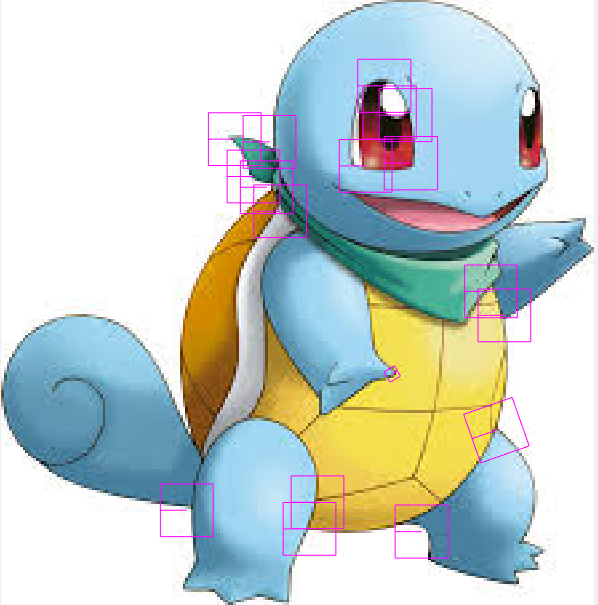
\includegraphics[width=1\linewidth]{img/squirtle1}
		  \caption{Detecting Harris corners on an image.}
		  \label{fig:squirtle1}
\end{figure}

Non-maximum suppression has been implemented using the Matlab function $ordfilt2()$, which produces an ordered maximum filter to ensure a detected feature is also the largest observed feature in a given neighborhood. This helps narrow down the amount of returned corners.

\subsection{Feature Description}
After locating interest points in images, each given point must have some way to be described in order to detect similarly described features within another scene. This program utilizes 3 different feature descriptor methods, each with its pros and cons.

The first method, $GetBadFeatures()$, is the simplest of the feature descriptor methods and is clearly an ineffective approach. This approach merely extracts a non-rotated $5 \times 5$ image descriptor from neighboring pixels around a feature.

\begin{figure}[h]
	\centering
		  \centering
		  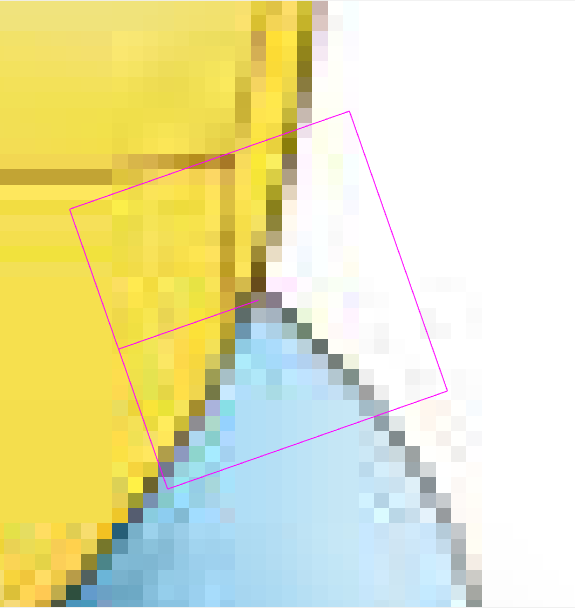
\includegraphics[width=1\linewidth]{img/squirtle2}
		  \caption{Enlarged feature descriptor from Figure~\ref{fig:squirtle1}}
		  \label{fig:squirtle2}
\end{figure}


The second attempt, $GetRotatedFeatures()$ attempts to detect features with an orientation implementation. After locating a particular feature, instead of extracting a standard $5 \times 5$ feature, a rotated $5 \times 5$ feature is extracted. The rotation is based on orientation calculations found from the image derivatives:

$$
Orientation(x,y) = atan( \frac{I_{y}}{I_{x}} )
$$

Where $I_{x}$ and $I_{y}$ are the $x$ and $y$ derivatives of an image, respectively.

The final implementation, $GetSIFTy()$, is the most accurate feature descriptor function. This is an algorithm similar to the one used in SIFT, with a few differences.
In this program, a $16 \times 16$ neighborhood surrounding each discovered corner is extracted and subdivided into $4 \times 4$ subdivisions. Within each block, the feature orientation is calculated and normalized by a Gaussian. This provides a robust, 128-dimensional feature vector which can be utilized in feature matching.

This implementation works excellently on illumination invariant images. Figures~\ref{fig:car1}~and~\ref{fig:car2} demonstrate the algorithm's ability to detect features when images differ in illumination. This was done by normalizing the 128-dimensional feature vectors so that each value in the vector is within a 0 to 1 scale. This scaling effect should hold similar between two similar images, even if the illumination varies.

Rotation invariance appears to be somewhat inaccurate. Figures~\ref{fig:graf1}~and~\ref{fig:graf2} yield several successful results despite being differing scales, but there are still several failures in matching. The program does not calculate histograms for each $4 \times 4$ subdivision in the image, which would improve orientation matches. Figures~\ref{fig:wall1}~,~\ref{fig:wall2}~,~and~\ref{fig:wall3} also illustrate this error, as more errors are yielded as the second image has a greater skew factor from the first. However, Figure~\ref{fig:yose3} demonstrates a successful rotation test.



\subsection{Feature Matching}
Feature matching involves the use of the Sum of Squared Differences equation explained in Section~\ref{sub:featmat}. The SSD is performed between all the 128-dimensional feature vectors in the two images. Distances that yield low values are likely candidates for matches. The standard SSD function is located in the $SSD()$ method.

However, merely implementing the SSD is a naive approach because ambiguous matches can oftentimes be detected as false positives. Therefore, a second function, $SSDRatio()$ has also been implemented. The ratio test takes the best and second best distances from a given feature match to perform the ratio. The larger the returned ratio, the closer the best and second best distances are to one another, which increases the probability of making a false match. Rather than risk this, it is simply better to throw out the match entirely if it does not meet a specified ratio validation value. In this implementation, any $\frac{best}{2_{nd} best}$ ratio greater than $0.8$ is discarded.

A final SSD variation, $SSDCustom()$, takes the knowledge of the first two SSD calculations to make an even more filtered validation method. This SSD calculation is based off of the ratio method, but also implements a tolerance threshold on top of the ratio validation. This threshold automatically throws out any distance that is greater than a user-specified value. This filters out any matches that happen to pass from coincidentally similar features.

The feature matching implemented in this program has a lot of successful matchings, as noted in the Appendix of this paper. 

Figures~\ref{fig:graf1}~and~\ref{fig:graf2} has a decent number of matches, but the feature matching could be improved overall. An inspection of other potential distance algorithms could potentially yield better results than the SSD. The Sum of Absolute Differences (SAD) has also been looked at in one of the additional functions, but did not yield any noteworthy improvements. There could potentially be better options out there that could generate more successful matchings.

\section{Conclusion}
This project was an in depth analysis on the nuances of feature detection and matching. Throughout this analysis, discussion of successes and failures in the implementation have been noted. Improvements to the feature matching can be made by modifying the feature vectors to be more invariant to other image anomalies besides the ones proven to be handled in the benchmark images. Other distance evaluations could be tested to produce better feature match results as well. Overall, the benchmark images appeared to return a good amount of matched features from the implemented functions.

The repository containing the code discussed in this writeup can be found at {\url{https://github.com/jbrackins/feature_detection}}

\clearpage



% if have a single appendix:
%\appendix[Proof of the Zonklar Equations]
% or
%\appendix  % for no appendix heading
% do not use \section anymore after \appendix, only \section*
% is possibly needed

% use appendices with more than one appendix
% then use \section to start each appendix
% you must declare a \section before using any
% \subsection or using \label (\appendices by itself
% starts a section numbered zero.)
%


\appendices
\section{Image Results}
The remainder of the document is a gallery of image results produced by the feature matching code, as well as any noteworthy observations concluded from successful and unsuccessful matching attempts. Larger versions of all images results will be made available online at {\url{http://julianbrackins.me/computerscience/vision/vision_1proj}}

\begin{figure}[h]
	\centering
		  \centering
		  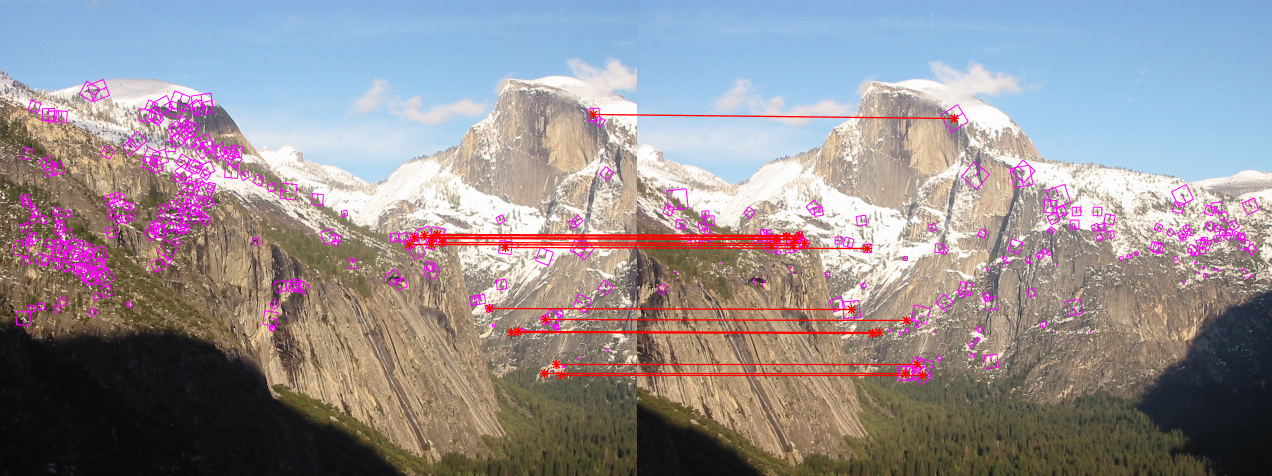
\includegraphics[width=1\linewidth]{img/yose1}
		  \caption{Feature Matching Yosemite image set. Success indicates feature matching works on translated images.}
		  \label{fig:yose1}
\end{figure}

\begin{figure}[h]
	\centering
		  \centering
		  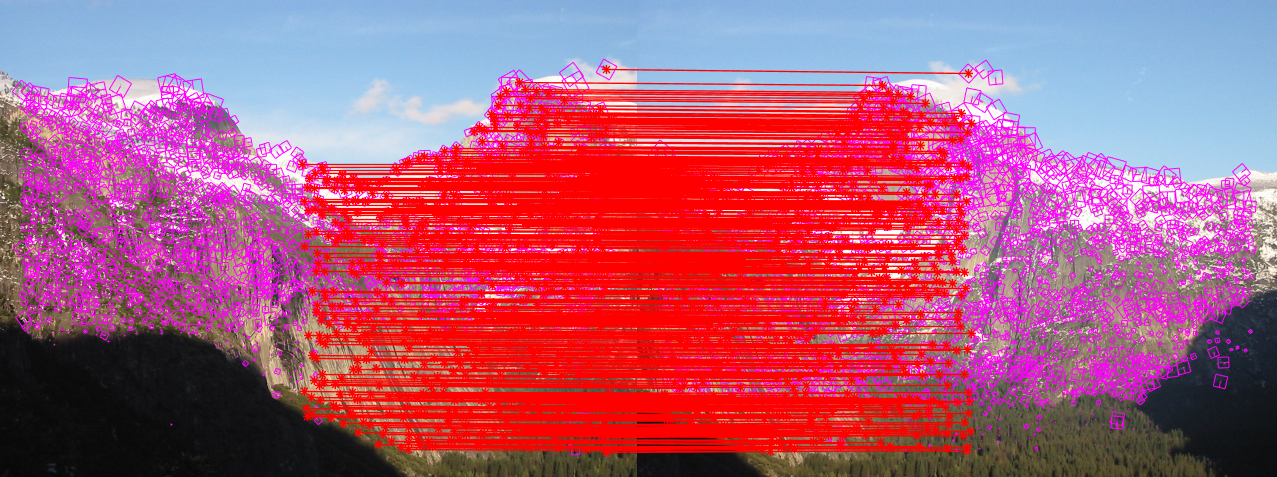
\includegraphics[width=1\linewidth]{img/yose2}
		  \caption{Robust Feature Matching Yosemite image set. Threshold value decreased in order to determine more image corners.}
		  \label{fig:yose2}
\end{figure}

\begin{figure}[h]
	\centering
		  \centering
		  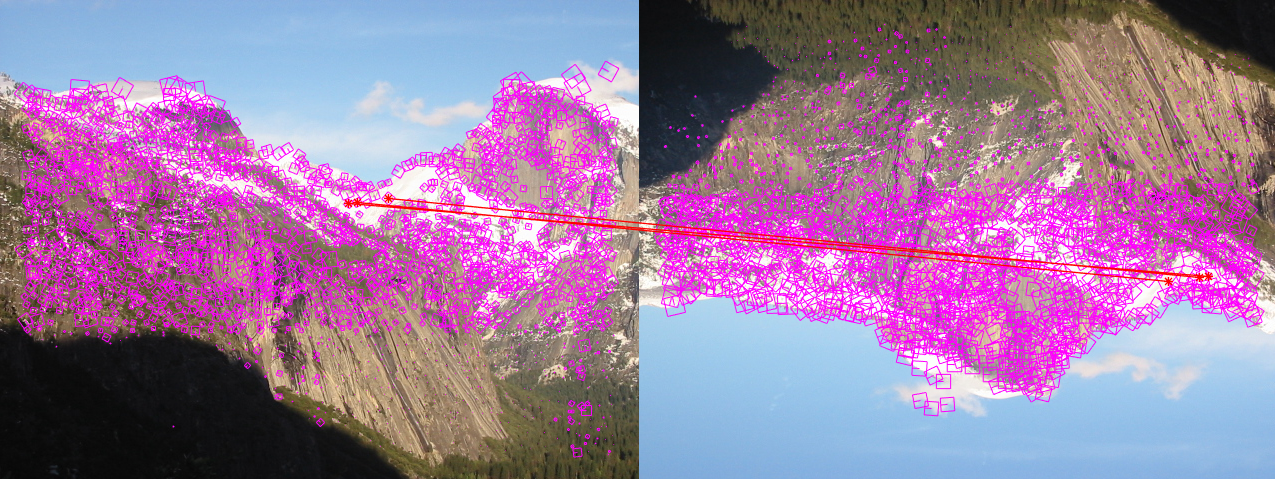
\includegraphics[width=1\linewidth]{img/yose3}
		  \caption{Feature Matching Yosemite image set with the second image rotated 180$^{\circ}$. Successful matched features indicate some level of rotation invariance in the program.}
		  \label{fig:yose3}
\end{figure}

\begin{figure}[h]
	\centering
		  \centering
		  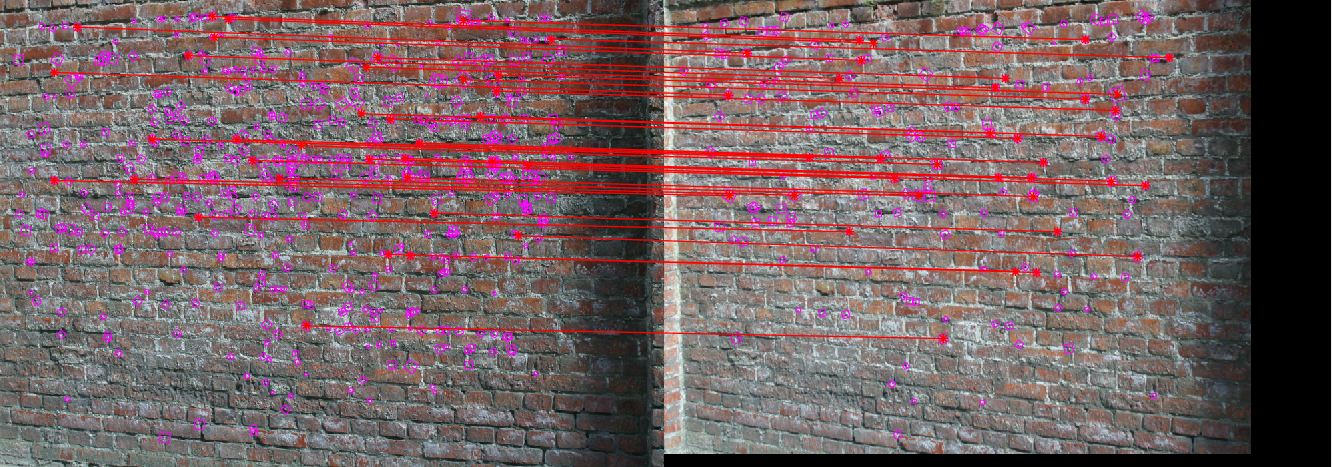
\includegraphics[width=1\linewidth]{img/wall1}
		  \caption{Feature Matching on wall images. Matched Features appear to be accurate.}
		  \label{fig:wall1}
\end{figure}

\begin{figure}[h]
	\centering
		  \centering
		  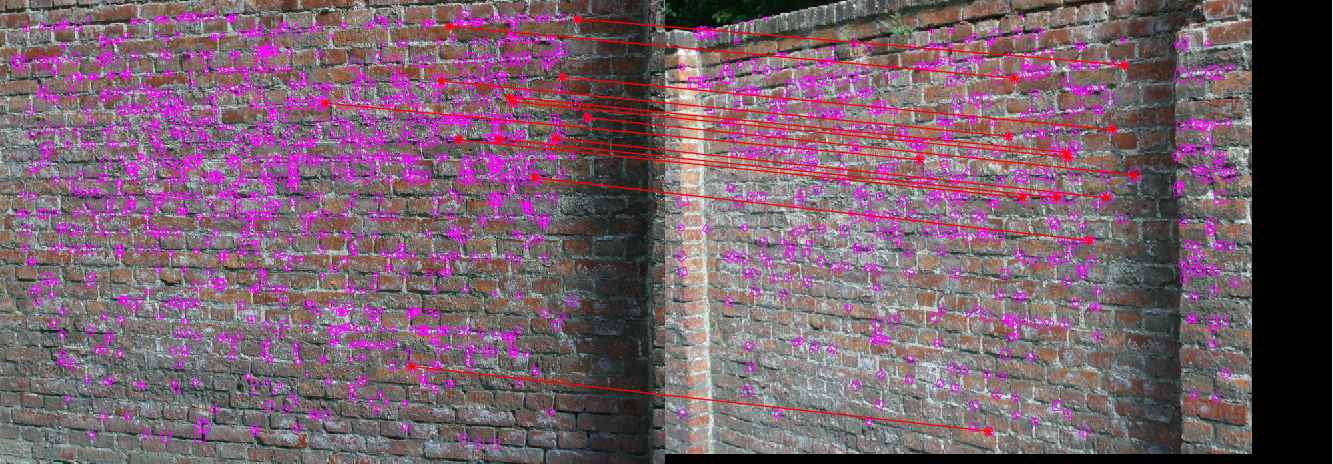
\includegraphics[width=1\linewidth]{img/wall2}
		  \caption{Feature Matching on wall images. Most matched features continue to appear accurate.}
		  \label{fig:wall2}
\end{figure}

\begin{figure}[h]
	\centering
		  \centering
		  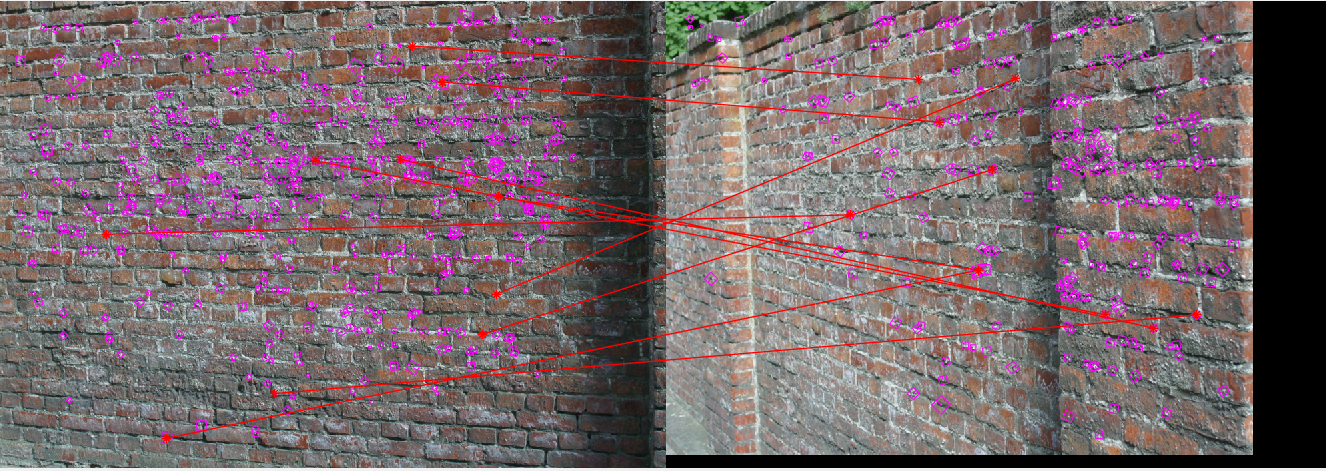
\includegraphics[width=1\linewidth]{img/wall3}
		  \caption{Feature Matching on wall images. Errors detected, but still maintains a few properly matched features.}
		  \label{fig:wall3}
\end{figure}


\begin{figure}[h]
	\centering
		  \centering
		  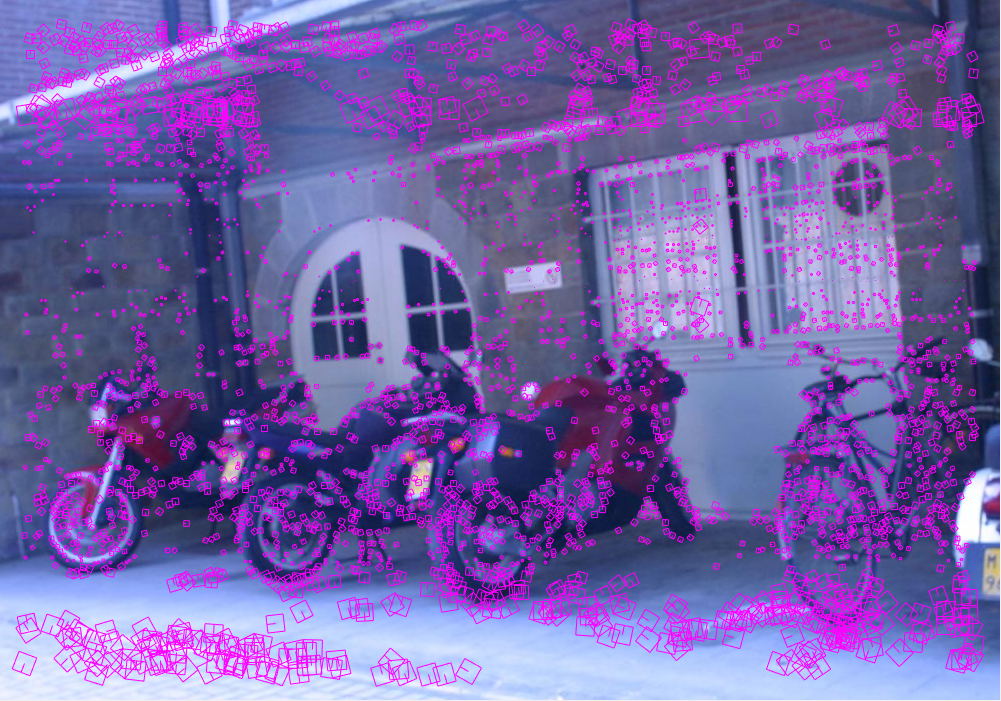
\includegraphics[width=1\linewidth]{img/bikes2b}
		  \caption{Feature Description on Bikes}
		  \label{fig:bikes2}
\end{figure}


\begin{figure}[h]
	\centering
		  \centering
		  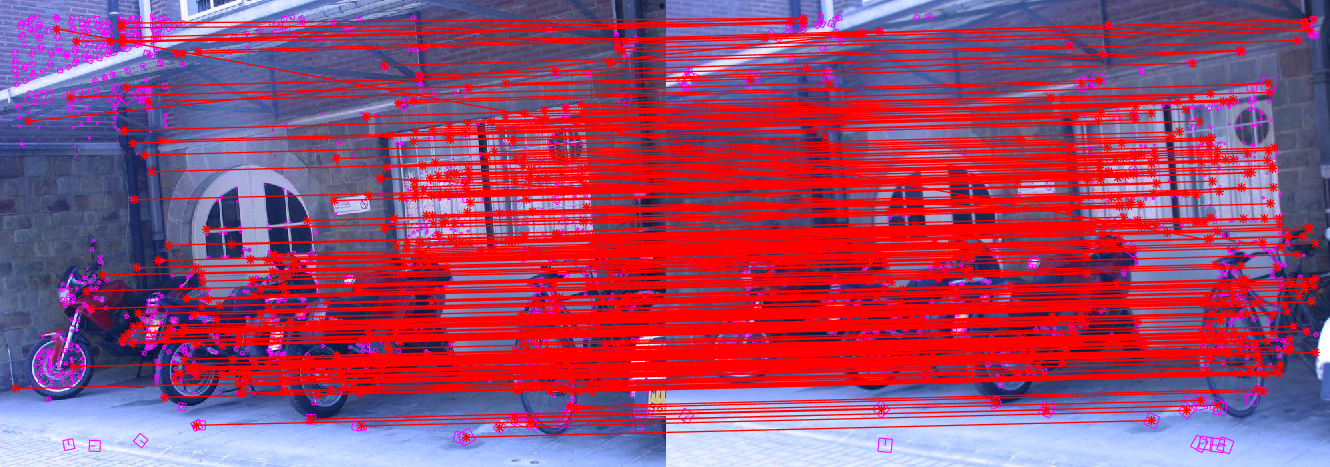
\includegraphics[width=1\linewidth]{img/bikes1}
		  \caption{Feature Matching on bikes with lowered threshold. A substantial increase in matched features is observed}
		  \label{fig:bikes1}
\end{figure}



\begin{figure}[h]
	\centering
		  \centering
		  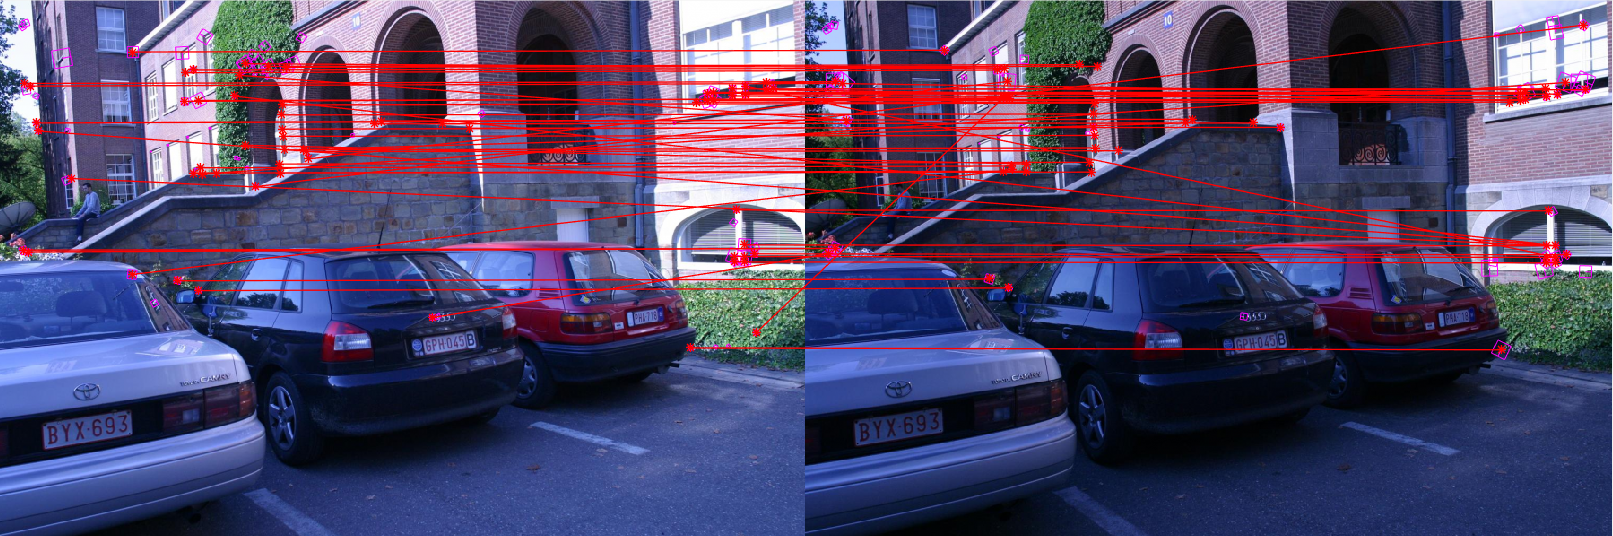
\includegraphics[width=1\linewidth]{img/car1}
		  \caption{Feature matching on leuven set.}
		  \label{fig:car1}
\end{figure}

\begin{figure}[h]
	\centering
		  \centering
		  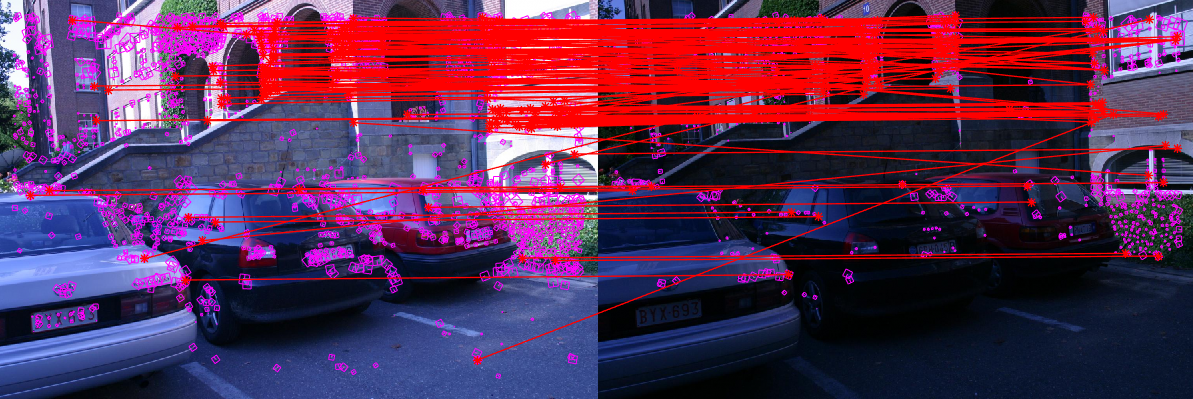
\includegraphics[width=1\linewidth]{img/car2}
		  \caption{Feature matching on leuven set with a darker second image. Illumination invariance observed with few errors.}
		  \label{fig:car2}
\end{figure}

\begin{figure}[h]
	\centering
		  \centering
		  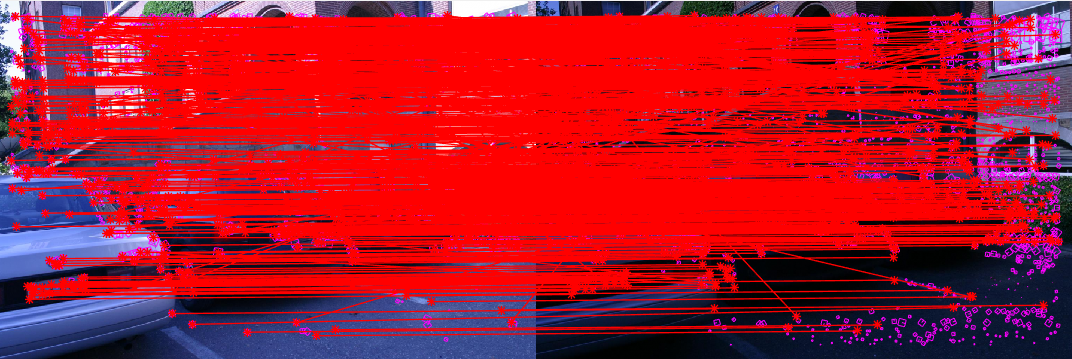
\includegraphics[width=1\linewidth]{img/car3}
		  \caption{Robust feature matching on leuven set.}
		  \label{fig:car3}
\end{figure}


\begin{figure}[h]
	\centering
		  \centering
		  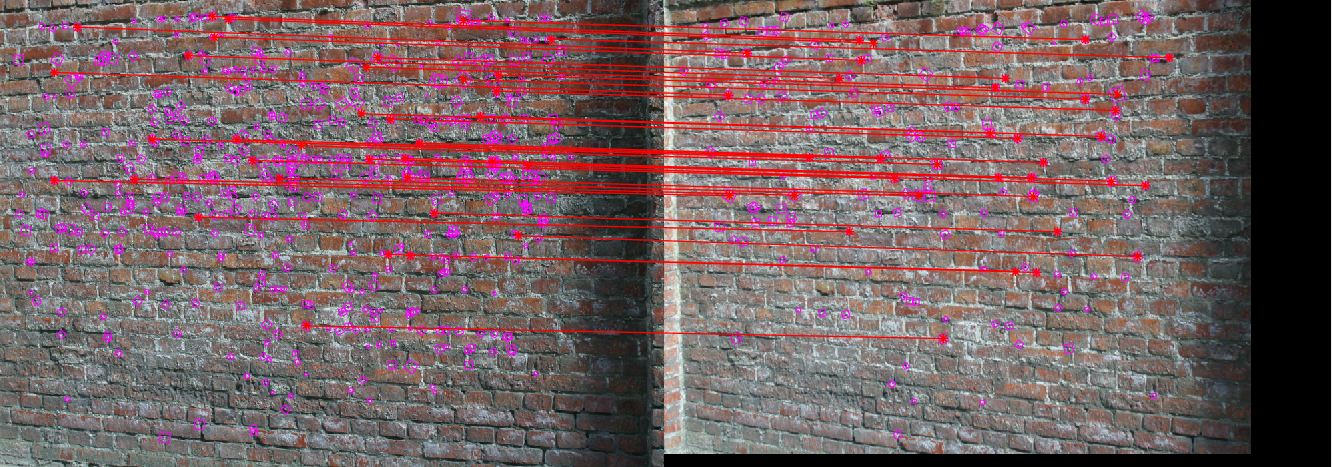
\includegraphics[width=1\linewidth]{img/wall1}
		  \caption{Feature Matching on wall images. Matched Features appear to be accurate.}
		  \label{fig:wall1}
\end{figure}

\begin{figure}[h]
	\centering
		  \centering
		  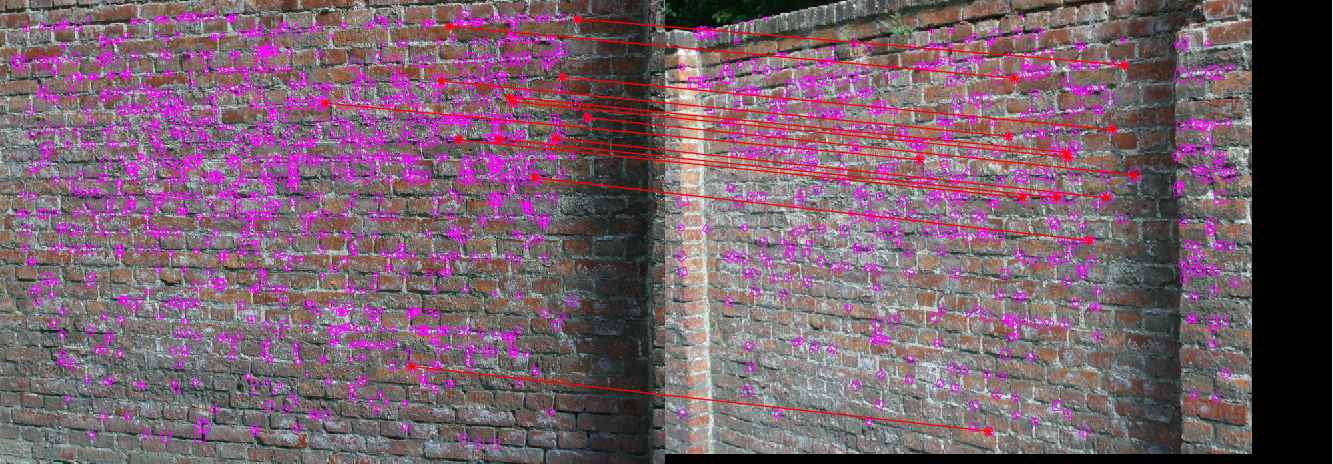
\includegraphics[width=1\linewidth]{img/wall2}
		  \caption{Feature Matching on wall images. Most matched features continue to appear accurate.}
		  \label{fig:wall2}
\end{figure}

\begin{figure}[h]
	\centering
		  \centering
		  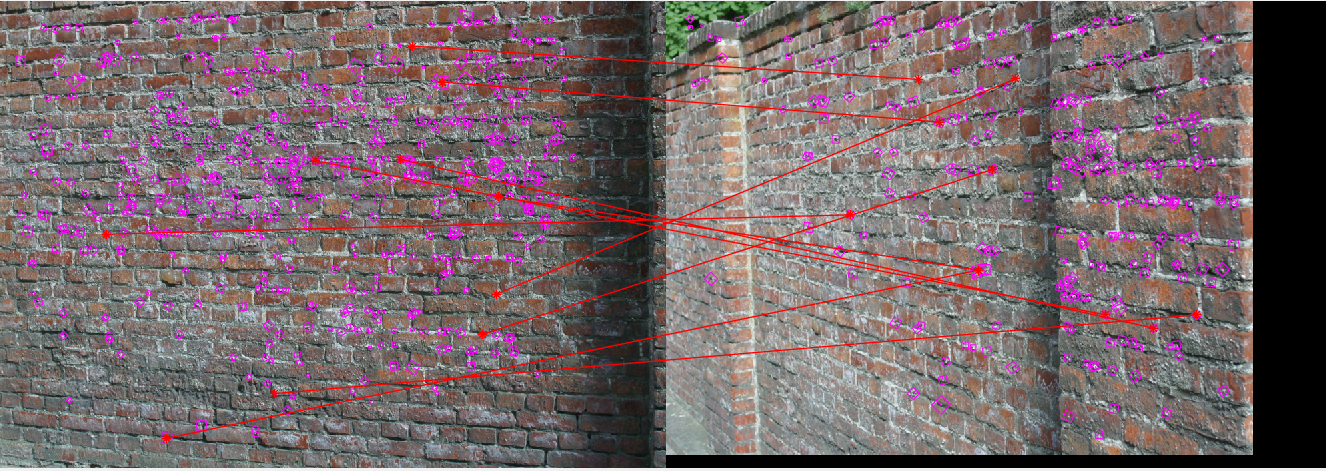
\includegraphics[width=1\linewidth]{img/wall3}
		  \caption{Feature Matching on wall images. Errors detected, but still maintains a few properly matched features.}
		  \label{fig:wall3}
\end{figure}

%%%%%%%%%%%%%%%%%

\begin{figure}[h]
	\centering
		  \centering
		  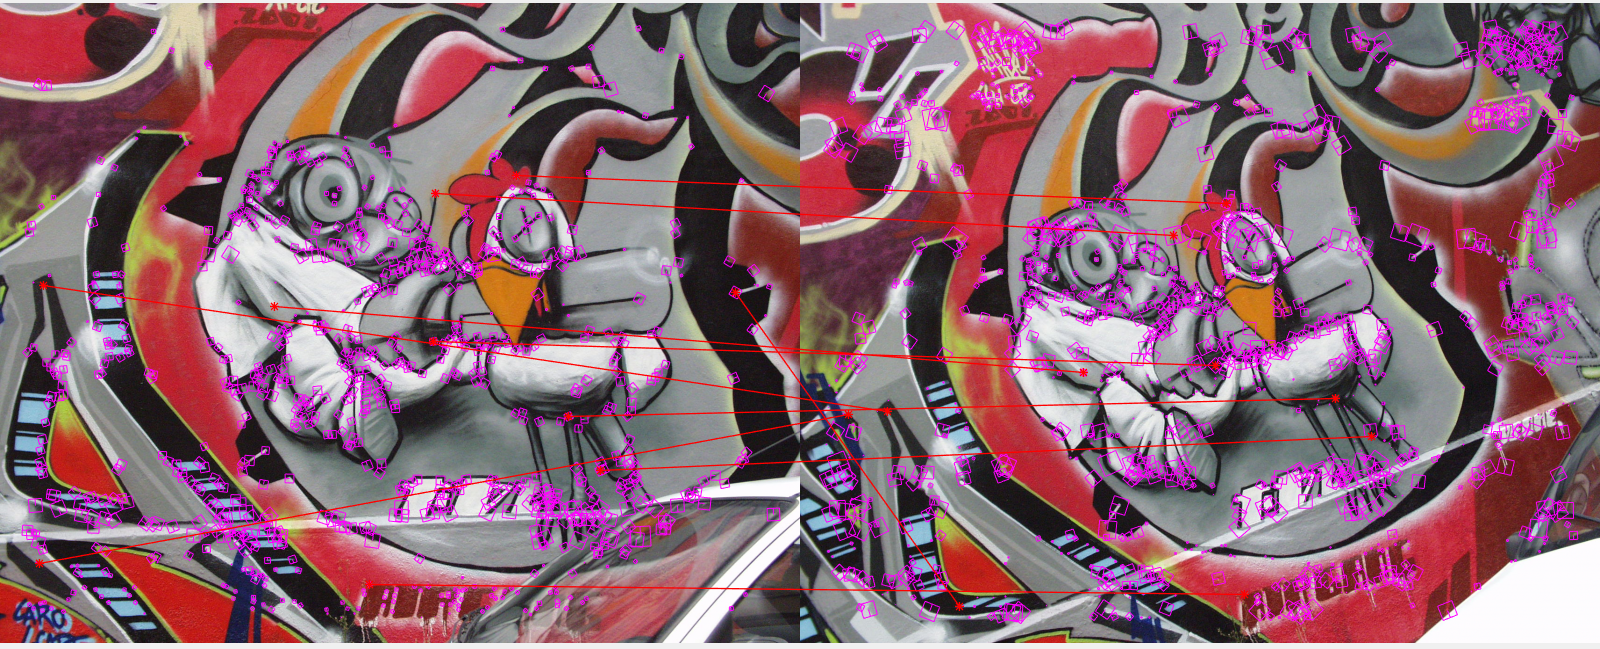
\includegraphics[width=1\linewidth]{img/graf1}
		  \caption{Feature Matching on graffiti set. Errors present but appears to have a number of successful matches}
		  \label{fig:graf1}
\end{figure}

\begin{figure}[h]
	\centering
		  \centering
		  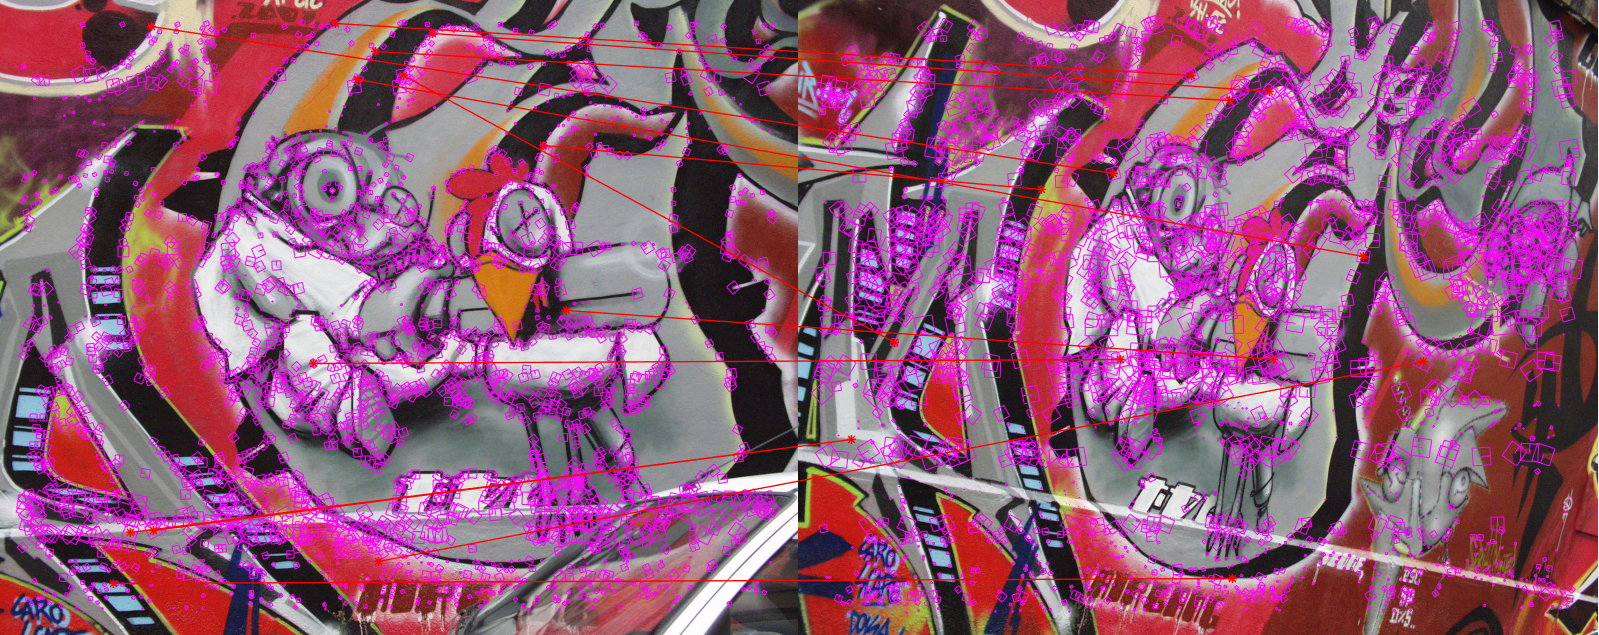
\includegraphics[width=1\linewidth]{img/graf2}
\caption{Feature Matching on graffiti set. Errors present still contains several matches despite noticeable image skew between pictures.}
		  \label{fig:graf2}
\end{figure}



% Can use something like this to put references on a page
% by themselves when using endfloat and the captionsoff option.
\ifCLASSOPTIONcaptionsoff
  \newpage
\fi



% trigger a \newpage just before the given reference
% number - used to balance the columns on the last page
% adjust value as needed - may need to be readjusted if
% the document is modified later
%\IEEEtriggeratref{8}
% The "triggered" command can be changed if desired:
%\IEEEtriggercmd{\enlargethispage{-5in}}

% references section

% can use a bibliography generated by BibTeX as a .bbl file
% BibTeX documentation can be easily obtained at:
% http://www.ctan.org/tex-archive/biblio/bibtex/contrib/doc/
% The IEEEtran BibTeX style support page is at:
% http://www.michaelshell.org/tex/ieeetran/bibtex/
%\bibliographystyle{IEEEtran}
% argument is your BibTeX string definitions and bibliography database(s)
%\bibliography{IEEEabrv,../bib/paper}
%
% <OR> manually copy in the resultant .bbl file
% set second argument of \begin to the number of references
% (used to reserve space for the reference number labels box)



% biography section
% 
% If you have an EPS/PDF photo (graphicx package needed) extra braces are
% needed around the contents of the optional argument to biography to prevent
% the LaTeX parser from getting confused when it sees the complicated
% \includegraphics command within an optional argument. (You could create
% your own custom macro containing the \includegraphics command to make things
% simpler here.)
%\begin{IEEEbiography}[{\includegraphics[width=1in,height=1.25in,clip,keepaspectratio]{mshell}}]{Michael Shell}
% or if you just want to reserve a space for a photo:



% insert where needed to balance the two columns on the last page with
% biographies
%\newpage



% You can push biographies down or up by placing
% a \vfill before or after them. The appropriate
% use of \vfill depends on what kind of text is
% on the last page and whether or not the columns
% are being equalized.

%\vfill

% Can be used to pull up biographies so that the bottom of the last one
% is flush with the other column.
%\enlargethispage{-5in}



% that's all folks
\end{document}


